\documentclass[11pt,letterpaper]{article}
\usepackage[utf8]{inputenc}
\usepackage[T1]{fontenc}
\usepackage[margin=1in]{geometry}
\usepackage{amsmath,amssymb}
\usepackage{graphicx}
\usepackage{hyperref}
\usepackage{xcolor}
\usepackage{enumitem}
\usepackage{caption}

\hypersetup{colorlinks=true,linkcolor=black,urlcolor=black,citecolor=black}
\graphicspath{{../figures/}}

\title{\textbf{Endangered Species Conservation in the Zoo Protocol}\\\large Routing Digital Economic Value to Real-World Wildlife}
\author{Antje Worring \\ \textit{Founder, Zoo Labs Foundation} \\ \texttt{antje@zoo.ngo}}
\date{October 31, 2021}

\begin{document}
\maketitle

\begin{abstract}
This element paper extracts the conservation thesis from the Zoo Whitepaper~\cite{zoo2021}. We document the V1 species roster, the population context for each, the on-chain mechanisms that route economic value to non-profit partners, and the educational pipeline operated by the Zoo Foundation in collaboration with K--12 schools.
\end{abstract}

\section{The V1 Species Roster}

The first Zoo drop catalogues species across three rarity tiers, each calibrated to the IUCN status and approximate wild population of the animal:

\begin{itemize}
  \item \textbf{Sublime} (5\% of distribution): Red Wolf (\textit{Canis rufus}). Approximately 35 individuals remain in the wild.
  \item \textbf{Rare} (15\% of distribution): Amur Leopard (under 70 wild individuals); Nubian Giraffe (under 2{,}645 wild individuals).
  \item \textbf{Endangered} (85\% of distribution): Sumatran Elephant; Pygmy Hippopotamus; Javan Rhinoceros (one wild population, none in captivity); Siberian Tiger ($\approx$500 wild individuals); Emperor Penguin (climate-imperilled).
\end{itemize}

The rarity-to-distribution mapping is intentional: the rarest digital animals correspond to species closest to extinction. Owning a Sublime Red Wolf is owning a digital twin of one of the rarest mammals on Earth.

\section{On-Chain Mechanisms}

The whitepaper specifies two primary value-routing mechanisms:

\begin{enumerate}
  \item \textbf{Sustainability tax on burn.} When an NFT is burned to release collateral and rewards, a 20\% sustainability tax applies: 10\% to the DAO, 10\% to the liquidity pool. The DAO then directs a portion of treasury inflows to non-profit partners.
  \item \textbf{Transaction tax on trades.} A small fee on collateral additions and on transactions in the Zoo ecosystem flows to the Zoo Labs Foundation~\cite{zoo2021}, supplemented by a 4\%/4\% split (DAO / liquidity) on the broader transaction set described in the Metaverse Companion section.
\end{enumerate}

These mechanisms make the conservation flow durable: it does not depend on philanthropic mood. Every economically motivated user, every speculator, every DeFi yield-farmer is routing value to the conservation treasury simply by participating.

\section{Non-Profit Partner Selection}

The DAO selects non-profit partners that satisfy three criteria:

\begin{itemize}
  \item Direct on-the-ground work with the species represented in the Zoo NFT roster.
  \item Public, audited financials.
  \item Willingness to publish impact reports that the Zoo community can verify.
\end{itemize}

The DAO publishes the partner list and the funding allocations. Members of the community can propose new partners, with proposals advancing through the standard governance process.

\section{Educational Pipeline}

The Zoo Foundation operates an educational pipeline complementary to the on-chain conservation flow:

\begin{itemize}
  \item Open-source curriculum aligned to K--12 learning standards in the United States.
  \item Free distribution to schools that opt in.
  \item Repository of student outputs, encouraging schools to share their work back to the open commons.
\end{itemize}

This pipeline begins shipping in Q2 2022~\cite{zoo2021}. The Foundation's resident Director of Education curates the materials.

\section{Animal Sanctuary}

A long-term Zoo Foundation goal is the establishment of physical animal sanctuaries open to local visitors and educators, where the digital twin economics literally fund the physical refuge for the species. The sanctuary is a tangible bridge between the digital ownership of an animal NFT and the physical preservation of its real-world counterpart.

\section{Why This Is Not Greenwashing}

The whitepaper takes pains to ground the conservation thesis in mechanism rather than marketing. Three specifics:

\begin{enumerate}
  \item \textbf{Public partner list and disbursements.} Every dollar (or token) routed to a non-profit is on chain. There is no private back-channel.
  \item \textbf{No central control over the flow.} The DAO --- not the Foundation directors --- ratifies disbursements. Founders cannot redirect the conservation treasury without a community vote.
  \item \textbf{Partnership with credentialed organizations.} Non-profits are vetted for direct work on the species; not generic environmental organizations.
\end{enumerate}

\begin{figure}[h]
\centering
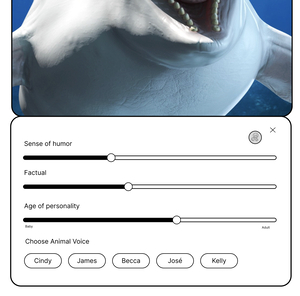
\includegraphics[width=0.32\textwidth]{whale.png}
\hspace{0.04\textwidth}
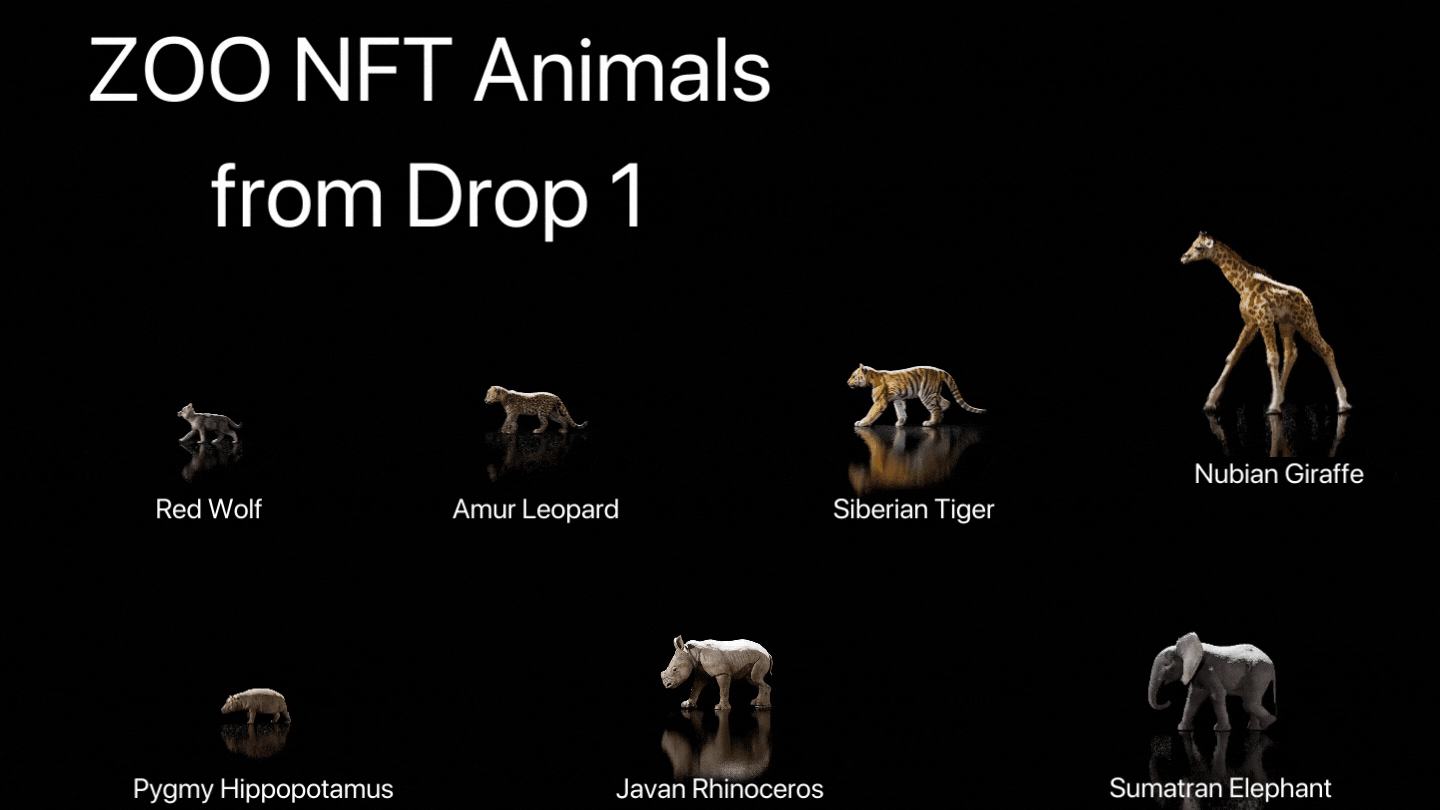
\includegraphics[width=0.55\textwidth]{animals.png}
\caption{Left: Whale, one of the species in the broader Zoo roster. Right: V1 animal lineup --- the digital twins whose economics fund the conservation of their real-world counterparts.}
\end{figure}

\section{Sustainability of the Crypto Layer Itself}

Conservation framing must also account for the environmental footprint of the underlying chain. The whitepaper~\cite{zoo2021} cites independent research showing that proof-of-stake (and the broader category of low-energy consensus) consume only a fraction of the energy used by traditional banking. Zoo's deployment plan deliberately targets low-energy chains and bridges:

\begin{itemize}
  \item Initial token launch on Binance Smart Chain to leverage low gas fees and a large existing user base.
  \item Cross-chain bridge to Ethereum (and beyond) for liquidity and composability without locking value in vault contracts.
  \item Future migration path to a Lux Layer-1 validator that further reduces per-transaction energy.
\end{itemize}

The combination of efficient consensus and economically routed conservation revenue is what allows Zoo to be a \emph{net positive} for the environment.

\section{Education and the Foundation's Role}

The Zoo Foundation~\cite{zoo2021} was established to harness blockchain technology and the global community it connects to help preserve our world's most critically endangered animal species. The Foundation's stated commitments include:

\begin{itemize}
  \item Creating digital twins of endangered species to raise awareness and enact change.
  \item Providing financial and human support to wildlife conservation partners.
  \item Hosting fundraising events with conservation partners and other strategic partners.
  \item Mitigating the devastating effects of the illegal wildlife trade by raising awareness and channeling resources toward law-enforcement-friendly partner organizations.
  \item Creating sustainable physical animal sanctuaries that double as educational venues for the local community.
\end{itemize}

These commitments are made institutional through the Foundation's status: it is the legally constituted vehicle through which the on-chain conservation flow becomes off-chain action.

\section{Conservation Funnel: From Holder to Habitat}

The end-to-end funnel from an NFT mint to a real-world habitat is:

\begin{enumerate}
  \item User mints or trades an NFT animal. A small fee is collected.
  \item The fee splits between liquidity-pool sustainment and the DAO treasury.
  \item DAO members vote on quarterly disbursement proposals listing specific non-profit partners and amounts.
  \item Disbursements are recorded on chain, then converted to fiat where required and wired to the partner organization.
  \item Partner organization publishes an impact report --- field projects funded, habitat preserved, anti-poaching patrols enabled.
  \item The community verifies and ratifies the report; future allocations to that partner are weighted accordingly.
\end{enumerate}

Each step in this funnel is auditable. There is no opaque step where money disappears into ``general operating expenses.''

\section{Long-Term Vision}

Beyond the V1 species roster, the long-term vision is for the Zoo ecosystem to support digital twins for as many of the 18{,}000 globally endangered species as the community ratifies. Each new species drop is a chance to fund another conservation partner, expand the educational catalogue, and bring another corner of the natural world into the consciousness of the broader public.

\begin{thebibliography}{1}
\bibitem{zoo2021} Antje Worring. \emph{Zoo: A Game-Fi Multiverse Ecosystem for the Preservation of Endangered Species}. Zoo Labs Foundation, October 31, 2021.
\end{thebibliography}

\end{document}
